Solve this by letting $u(x, t) = u_s(x) + v(x, t)$, where $u_s(x)$ is the steady state solution and $v(x, t)$ is the
transient solution.

\begin{solution}\ \\\\
    We assume the full solution $u(x, t)$ to our system is the sum of a steady state function $u_s(x)$ and a transient 
    solution $v(x, t)$. We begin with the observation that the fact that the bar is insulated at $x = L$ and held at
    constant temperature at $x = 0$ implies that the steady state temperature ought to settle to that of the constant
    temperature of $10^{\circ}$ for all $x \in [0, L]$. To show this mathematically, we observe that in the steady state
    scheme, the temperature does not change with respect to time and hence our heat equation reduces to:

    $$
    u_{xx} = 0
    $$

    We integrate the above equation twice to find that the steady state solution is given by $u_s(x) = ax + b$ for some
    constants $a$ and $b$. In the steady state scheme, our transient solution is by definition 0, and hence our Neumann
    boundary condition implies

    $$
    0 = u_x(L, t) = (u_s + 0)_x(L) = \left[\frac{\partial}{\partial x}(ax + b)\right](L) = a
    $$

    and hence $a = 0$. Similarly, our Dirichlet boundary condition yields:

    $$
    10 = u(0, t) = (u_s + 0)(0, t) = u_s(0) = b
    $$

    and therefore our steady state solution is simply:

    \begin{equation}
        u_s(x) = 10
    \end{equation}

    We now solve for the transient solution $v(x, t)$.  To do so, we utilize separation of variables and 
    assume that $v(x, t)$ is the product of some function of $x$ and some function of $t$, i.e., 
    $v(x, t) = \phi(x) G(t)$. Substituting the product form of $v(x, t)$ into the heat equation yields:

    $$
    \frac{\partial^2}{\partial x^2} (\phi(x) G(t)) = \frac{\partial}{\partial t} (\phi(x) G(t)) \\
    $$

    and hence (observing that the partial derivatives on either side reduce to standard derivatives):

    $$
    G \frac{d^2 \phi}{d x^2} = \phi \frac{d G}{d t}.
    $$

    \pagebreak
    We divide both sides by $\phi G$ to find:

    $$
    \frac{1}{\phi} \frac{d^2 \phi}{d x^2} = \frac{1}{G} \frac{d G}{d t}.
    $$

    Since the left-hand side depends on $x$ only and the right-hand side on $t$, the left and right sides must be equal
    to some constant, which we denote $-\lambda^2$.

    The time-dependent side therefore becomes the first-order ODE:

    $$
    \frac{d G}{d t} = -\lambda^2 G.
    $$

    with solutions for any particular $\lambda$ given by:\footnote{
        We add subscripts here to $d_{\lambda}$ and $G_{\lambda}$ in order to emphasize that the exact form of the 
        function depends on the particular value which $\lambda$ takes.
    }

    $$
    G_{\lambda}(t) = d_{\lambda}e^{-\lambda^2 t}.
    $$

    Similarly, the space-dependent side becomes the following second-order ODE:

    $$
    \frac{d^2 \phi}{d x^2} = -\lambda^2 \phi.
    $$

    with the following general solution (where coefficient values again depend on $\lambda$):

    $$
    \phi(x) = b_{\lambda} \sin{(\lambda x)} + c_{\lambda} \cos{(\lambda x)}.
    $$

    We substitute our boundary condition $10 = u(0, t) = 10 + v_x(0, t)$ to find:

    $$
    10 = 10 + \phi(0) G(t) = 10 + \left[b_{\lambda} \sin{(0)} + c_{\lambda} \cos{(0)}\right] G(t) = 10 + c_{\lambda} G(t).
    $$

    Subtracting both sides by 10 and dividing by $G(t)$ yields:\footnote{
        Since $G(t)$ is an exponential, we have $G(t) \neq 0$.
    }

    $$
    c_{\lambda} = 0.
    $$

    At $x = L$, we have:

    $$
    0 = u_x(L, t) 
      = \phi_x(L) G(t) 
      = \left[\lambda b_{\lambda} \cos{(L)} - \lambda c_{\lambda} \sin{(L)}\right] G(t) 
      = \lambda b_{\lambda} \cos{(\lambda L)} G(t).
    $$

    Since we are looking to find non-trivial solutions, we assume $b_{\lambda} \neq 0$ (and recall that $G(t) \neq 0$).
    Hence $\lambda$ must satisfy:

    $$
    \cos{(\lambda L)} = 0
    $$

    This is achieved whenever $\lambda_n = \frac{(2 n - 1) \pi}{2L}$.

    Hence for any particular $n$, we have that $v_n(x, t) = \phi_n(x)G_n(t)$ is a solution to our PDE. Because arbitrary
    linear combinations of solutions are themselves solutions to the PDE by the principle of superposition, we have that
    our transient solution $v(x, t)$ is given by:\footnote{
        We reindex by letting $a_n = c_n d_n$.
    }

    \begin{equation}
    v(x, t) = \sum\limits_{n=1}^{\infty}{b_n \sin{(\lambda_n x)}} d_n e^{-\lambda_n^2 t}
            = \sum\limits_{n=1}^{\infty}{a_n \sin{(\lambda_n x)}} e^{-\lambda_n^2 t}
    \end{equation}

    where $\lambda_n = \frac{(2 n - 1) \pi}{2L}$. To determine our Fourier cosine coefficients $a_n$, we substitute (1)
    and (2) into our initial condition $u(x, 0) = 10 + x$:

    \begin{align*}
        10 + x = u(x, 0) = u_s(x) + v(x, 0) = 10 + \sum\limits_{n=1}^{\infty}{a_n \sin{(\lambda_n x)}}.
    \end{align*}

    We subtract 10 from each side, multiply by $\sin{(\lambda_m x)}$ for some fixed $m \in \mathbb{N}$, and 
    integrate over our domain $\Omega = [0, L]$ to find:\footnote{
        We may switch the order of integration and summation by the Dominated Convergence Theorem.
    } \footnote{
        It can be shown via sine identities that 
        $\int_0^L{\sin{(\lambda_m x)} \sin{(\lambda_n x)}}\; dx = \frac{L}{2} \delta_{mn}$ for 
        $\lambda_n = \frac{(2n - 1) \pi}{2L}$.
    }

    \begin{align*}
        \int_{0}^{L}{x \sin{\frac{(2 m - 1) \pi x}{2L}}\; dx}
            &= \int_{0}^{L}{\sum\limits_{n=1}^{\infty}{a_n \sin{\frac{(2 n - 1) \pi x}{2L}} \sin{\frac{(2 m - 1) \pi x}{2L}} }\; dx} \\
            &= \sum\limits_{n=1}^{\infty}{a_n \int_{0}^{L}{\sin{\frac{(2 n - 1) \pi x}{2L}} \sin{\frac{(2 m - 1) \pi x}{2L}} \; dx }} \\
            &= \frac{L}{2} a_m.
    \end{align*}

    Our Fourier cosine coefficients (for $m \ge 1$) are therefore given by:

    \begin{alignat*}{2}
        a_m &= \frac{2}{L} \int_{0}^{L}{x \sin{\frac{(2m - 1) \pi x}{2L}} \; dx} \\
            &= -\frac{4}{(2m - 1)\pi} x \cos{\frac{(2m - 1) \pi x}{2L}} \biggm\rvert_{0}^{L} 
               + \frac{4}{(2m - 1)\pi} \int_{0}^{L}{\cos{\frac{(2m - 1) \pi x}{2L}} \; dx}  \\
            &= 0 + \frac{8 L}{(2m - 1)^2 \pi^2} \sin{\frac{(2m - 1) \pi x}{2L} \biggm\rvert_{0}^{L} \; dx}  \\
            &= \frac{8L}{(2m - 1)^2 \pi^2} (-1)^{m+1}.
    \end{alignat*}

    \pagebreak
    Substituting this expression into (2) yields our full solution $u(x, t)$:
    
    \begin{align*}
    u(x, t) &= u_s(x) + v(x, t) \\
            &= 10 + \sum\limits_{n=1}^{\infty}{a_n \sin{\left(\lambda_n x\right)} e^{-\lambda_n^2 t}} \\
            &= 10 + \sum\limits_{n=1}^{\infty}{\frac{8 L}{(2n - 1)^2 \pi^2} (-1)^{n+1} \sin{\left[\frac{(2n - 1) \pi}{2L} x \right]} e^{-\left[ \frac{(2 n - 1) \pi}{2L} \right]^2 t}}
    \end{align*}

    % For completeness, we plot two Fourier Series approximations to $u(x, 0) = x$:

    % \begin{figure*}[h]
    %     \centering
    %     \begin{subfigure}[b]{0.475\textwidth}
    %         \centering
    %         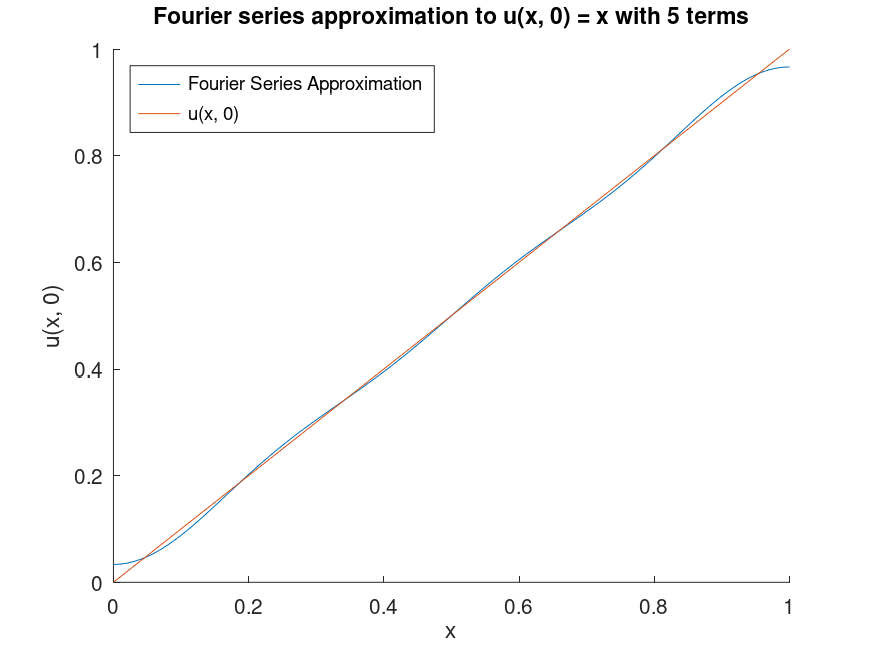
\includegraphics[width=\textwidth]{problem1_initial_fourier_series_solution_5_terms.png}
    %         \label{fig:problem1_5terms}
    %     \end{subfigure}
    %     \hfill
    %     \begin{subfigure}[b]{0.475\textwidth}
    %         \centering
    %         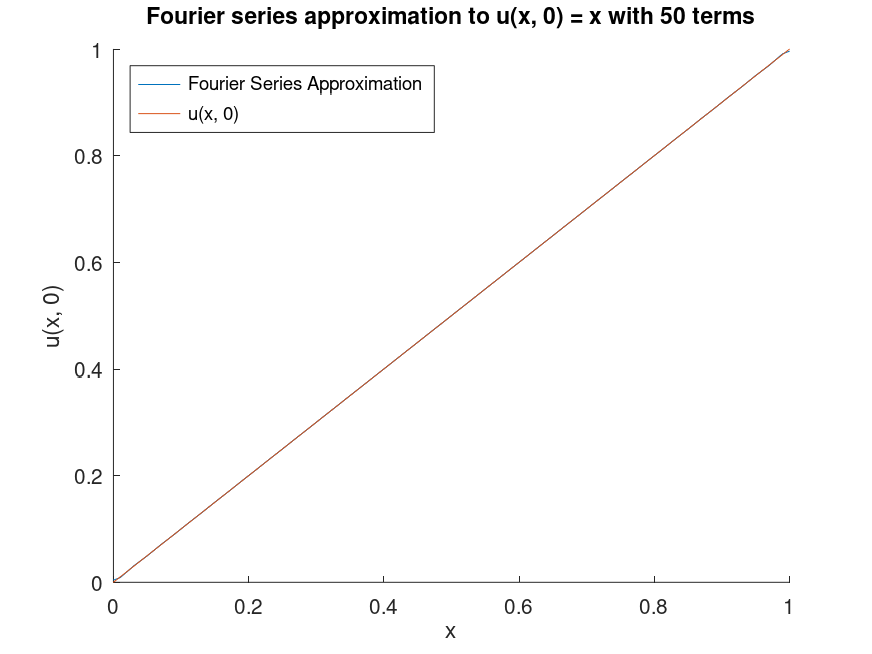
\includegraphics[width=\textwidth]{problem1_initial_fourier_series_solution_50_terms.png}
    %         \label{fig:problem1_50terms}
    %     \end{subfigure}
    %     \caption[Fourier Series solution]
    %     {\small Fourier Series approximation to $u_0(x) = x$} 
    %     \label{fig:fouriersoln}
    % \end{figure*}

    % \pagebreak

    % Lastly, observe that as $t$ gets large, the dominant term in the series is at $n=1$ (i.e., 
    % $-\frac{4}{\pi^2} \cos{(\pi x) e^{-\pi^2 t}}$) since the contribution from all even terms is zero and each 
    % successive odd term is exponentially smaller than the last. In fact, even for $t = 0.2$ we see negligible 
    % difference between 1 term and 255 terms:
    % \ \\\\

    % \begin{figure*}[h]
    %     \centering
    %     \begin{subfigure}[b]{0.475\textwidth}
    %         \centering
    %         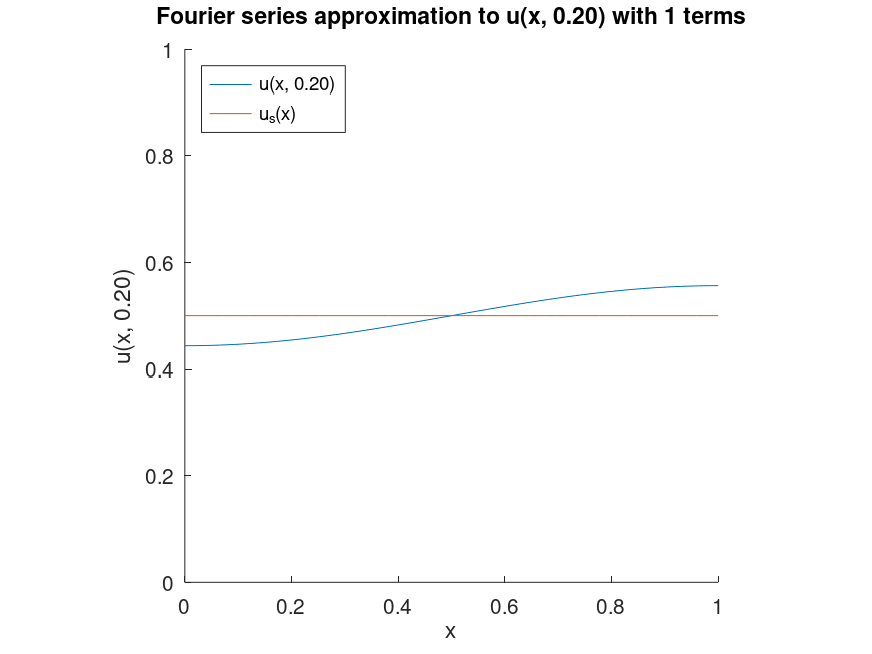
\includegraphics[width=\textwidth]{problem1_fourier_series_solution_1_terms_t_0.20.png}
    %         \label{fig:problem1_time_dependent_1term}
    %     \end{subfigure}
    %     \hfill
    %     \begin{subfigure}[b]{0.475\textwidth}
    %         \centering
    %         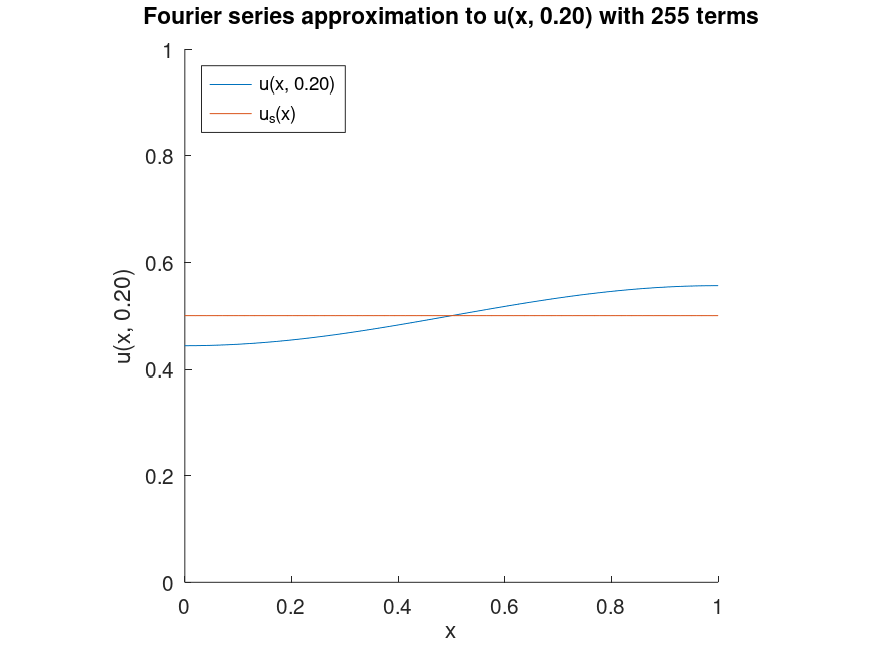
\includegraphics[width=\textwidth]{problem1_fourier_series_solution_255_terms_t_0.20.png}
    %         \label{fig:problem1_time_dependent_255terms}
    %     \end{subfigure}
    %     \caption[Fourier Series solution at $t = 0.2$]
    %     {\small Fourier Series approximation at $t = 0.2$} 
    %     \label{fig:fouriersoln}
    % \end{figure*}
    \ \\
\end{solution}